\documentclass{article}

\usepackage{amsthm,amsmath,amssymb}
\usepackage[numbers]{natbib}
\usepackage{hyperref}
\usepackage{graphicx}
\usepackage{caption}
\usepackage{subcaption}
\newcommand{\bx}{{\mathbf x}}
\newcommand{\ba}{{\mathbf a}}
\newcommand{\bv}{{\mathbf v}}
\newcommand{\bu}{{\mathbf u}}


\newtheorem{theorem}{Theorem}[section]
\newtheorem{proposition}[theorem]{Proposition}
\newtheorem{lemma}[theorem]{Lemma}
\newtheorem{corollary}[theorem]{Corollary}
\newtheorem{remark}{Remark}[section]
\newtheorem{example}[theorem]{Example}


\begin{document}

\title{Management Sciences Topics: Convex Optimization\\ Homework 2: Due Feb 21 (11:59 pm) }
%\author{Qihang Lin}
\date{}

\maketitle
\noindent(You can directly use any properties, theorems, examples or facts from the lectures.)
\bigskip

\noindent\textbf{Problem 1:}  What are the KKT conditions and the dual problems of the following minimization problems?
\begin{enumerate}
\item[a.] $\min_{x,y} c_1^\top x+c_2^\top y~\text{ s.t. }~Ax+By\leq d,~x\geq0$, where $c_1\in\mathbb{R}^{d_1}$, $c_2\in\mathbb{R}^{d_2}$, $A\in\mathbb{R}^{p\times d_1}$, $B\in\mathbb{R}^{p\times d_2}$ and $d\in\mathbb{R}^p$.

The dual problem:
$$
\begin{aligned}
\text{maximize}\quad &g(\lambda, \nu) = \inf_{x\in \mathcal{D}} c_1^\top x + c_2^\top y +  \lambda_1(Ax+By-d) +\lambda_2(-x),
\\
\text{subject to}\quad &\lambda\succeq 0.
\end{aligned}
$$
where $\mathcal{D} = \{(x, y)\mid Ax+By \le d, x\ge 0\}$.

The KKT conditions:
$$
\begin{aligned}
A\tilde{x}+B\tilde{y}-d &\le 0, \\
-\tilde{x} &\le 0, \\
\tilde\lambda_i &\ge 0, \ i = 1, 2 \\
\tilde\lambda_1(Ax+By-d) &= 0, \\
\tilde\lambda_2 \tilde{x} &= 0, \\
\begin{pmatrix}
c_1 \\ c_2
\end{pmatrix}
+
\tilde\lambda_1
\begin{pmatrix}
A \\ B
\end{pmatrix}
+\tilde\lambda_2
\begin{pmatrix}
-1_x \\ 0
\end{pmatrix}
&= 0.
\end{aligned}
$$

\item[b.] $\min_{x\in\mathbb{R}^d}\frac{1}{2}x^\top Px+q^\top x ~\text{ s.t. }~Ax\leq b$, where $P\in\mathbb{R}^{d\times d}$, $q\in\mathbb{R}^d$, $A\in\mathbb{R}^{p\times d}$, $b\in\mathbb{R}^p$ and $P$ is a positive definite (and thus invertible) symmetric matrix.

The dual problem:
$$
\begin{aligned}
\text{maximize}\quad &g(\lambda, \nu) = \inf_{x\in \mathcal{D}} \frac{1}{2}x^\top Px + q^\top x + \lambda (Ax-b)
\\
\text{subject to}\quad &\lambda\succeq 0.
\end{aligned}
$$
where $\mathcal{D} = \{x\mid Ax\le b\}$.

The KKT condition:
$$
\begin{aligned}
A\tilde{x} - b &\le 0, \\
\tilde\lambda &\ge 0,  \\
\tilde\lambda(A\tilde{x} - b) &= 0, \\
P\tilde{x}+q +\tilde{\lambda}A &= 0.
\end{aligned}
$$

\end{enumerate}

\noindent\textbf{Problem 2:} Do the following problems satisfy Slater's condition? Does strong duality ($d^*=p^*$) hold for these problems? You only need to answer Yes or No for both questions. (Note that $d^*=p^*$ holds when they are both $+\infty$ or both $-\infty$.)
\begin{enumerate}
	\item[a.]  $\min_{x\in\mathbb{R}} \exp(-x)\text{ s.t. }x=0$.

	Satisfy Slater's condition, and strong duality holds.

	\item[b.]  $\min_{x\in\mathbb{R}} \exp(-x)\text{ s.t. }x^2\leq0$.

	Does not satisfy Slater's condition, strong duality holds.

	\item[c.]  $\min_{x\in\mathbb{R}} x\text{ s.t. }x\leq-1, x\geq 1$.

	Does not satisfy Slater's condition, strong duality holds.

\end{enumerate}
\bigskip

\noindent\textbf{Problem 3:} Consider the following problem of projecting $z\in\mathbb{R}^d$ to a simplex:
\begin{eqnarray*}
	\min_{x}&& \frac{1}{2}\|x-z\|_2^2\\
	\text{s.t.}&& \sum_{i=1}^dx_i=1\\
	&& x_i\geq 0, \quad i=1,\dots,d.
\end{eqnarray*}
Answer the following questions:
\begin{enumerate}
\item[a.] For $r\in\mathbb{R}$, let $x_i(r):=\max\{z_i-r,0\}$ and $H(r):=\sum_{i=1}^d x_i(r)$. Show that there must be a $r^*$ such that $H(r^*)=1$. (Hint: Show that $H(r)$ is non-increasing in $r$ and $H(r)\rightarrow 0$ as $r\rightarrow+\infty$ and $H(r)\rightarrow +\infty$ as $r\rightarrow-\infty$.)

\begin{proof}
First, for $r_1 < r_2 $, 
$$
H(r_1) = \sum_{i=1}^{d}x_i(r_1) = \sum_{i=1}^{r}\max\{z_i-r_1, 0\} \ge \sum_{i=1}^{r}\max\{z_i-r_2, 0\} = H(r_2),
$$
so $H(r)$ is nonincreasing. As $r\to+\infty$, $z_i - r < 0$ for some $r > \max\{z_i\}$. Hence $H(r)\to 0$ for $r\to+\infty$. On the other hand, when $r\to-\infty$, $z_i-r > -|z_i|-r\to+\infty $. Hence $H(r)\to+\infty$. Notice $H(r)$ is continuous in $r$, there is a $r^* $, s.t. $H(r^*) = 1$.

\end{proof}

\item[b.] Let $r^*$ defined as in question a. Show that $x_i^*=x_i(r^*)=\max\{z_i-r^*,0\}$ is the optimal solution. To do that, you need to find the corresponding dual variables which satisfy the KKT conditions together with $x^*$.

\begin{proof}
Consider the dual problem
$$
\begin{aligned}
\max\quad &\frac{1}{2}\lVert x-z\rVert_2^2 - \sum_{i=1}^{d}\lambda_ix_i + \nu (\sum_{i=1}^{d}x_i - 1), \\
\text{s.t.}\quad &\lambda \succeq 0,
\end{aligned}
$$
and the KKT conditions
$$
\begin{aligned}
x_i &\ge 0, \quad i = 1,\hdots, d, \\
\sum_{i=1}^{d}x_i &= 1, \\
\lambda_i &\ge 0, \quad i = 1,\hdots, d, \\
\lambda_ix_i &= 0, \quad i = 1,\hdots, d, \\
\begin{pmatrix}
x_1-z_1 \\ \vdots \\ x_d-z_d
\end{pmatrix}
-
\begin{pmatrix}
\lambda_1 \\ \vdots \\ \lambda_d
\end{pmatrix}
+\nu
\begin{pmatrix}
1 \\ \vdots \\ 1
\end{pmatrix}
&= 0.
\end{aligned}
$$
 
Now we show the solution $x = x^* $ satisfies the KKT condition. Notice $\sum_{i=1}^{d}x_i^* = 1 $, so there must be an index $i$, s.t. $x_i^* > 0 $. Then for this $x_i^* $, $\lambda_i = 0 $, so $\nu = z_i - x_i^* = r^* $. Now consider $x_j^* = 0 $, then $\lambda_j = \nu - z_j = r^* - z_j \ge 0 $. Hence $(\lambda^*, \nu^*, x^*)$ satisfies the KKT condition, and hence $x^* $ is the optimal solution.

\end{proof}

\end{enumerate}
\bigskip

\noindent\textbf{Problem 4:} Implement the Proximal Gradient (PG) method to solve the following problems defined on the datasets from the LIBSVM library. You need to submit exactly two matlab files for each problem, one for the PG method without line search and one for the PG method with line search.
You need to initialize both algorithms at $\bx=\mathbf{0}$. In the PG method without line search, you need to manually tune $\eta$ to obtain a reasonably good convergence speed. In the PG method with line search, you need to choose $\eta_0=1$, $\gamma_{\text{inc}}=0.5$, and $\gamma_{\text{dec}}=0.5$. Run the PG method for 200 iterations for each problem and plot the objective value at each iteration. 
\begin{enumerate}
\item[a.] Box-constrained linear regression: $\min\limits_{\bx\in\mathbb{R}^d} \frac{1}{2}\|Ax-b\|_2^2$ s.t. $-10\leq x_i\leq 10$. $(b,A)$ is from E2006-tfidf (the one we showed in the class).
\item[b.] $\ell_1$-ball-constrained logistic regression: $\min\limits_{\bx\in\mathbb{R}^d} \frac{1}{n}\sum_{i=1}^n\log(1+\exp(-b_i(\ba_i\top\bx)))$ s.t. $\|\bx\|_1\leq 10$. Here, $b_i\in\{1,-1\}$ is the class label. Dataset: rcv1.binary. You can directly use the Matlab code by John Duchi (\url{https://stanford.edu/~jduchi/projects/DuchiShSiCh08.html}) for projections onto the $\ell_1$-ball. 
\end{enumerate}

The codes are in the ``codes'' subfolder, where the \texttt{box\_constrained\_linear\_regression} is the code for problem (a), and \texttt{l1\_constrained\_logistic\_regression} is for problem (b). The results are as follows:

\begin{figure}[h]
\centering
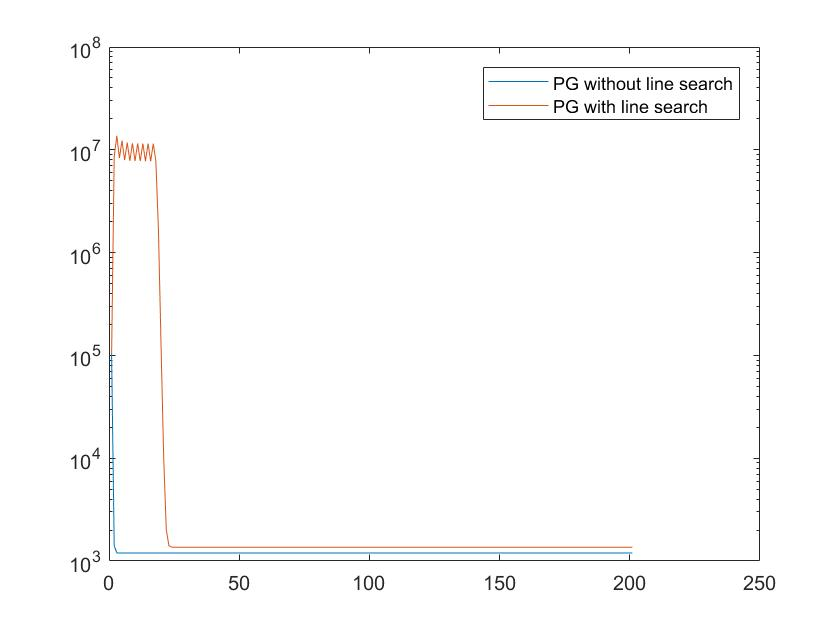
\includegraphics[scale=0.4]{a.jpg}
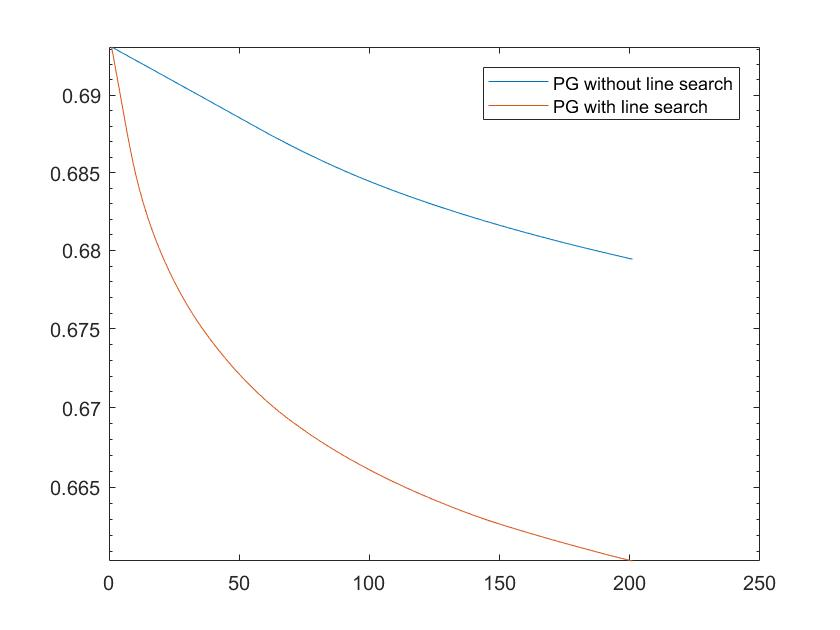
\includegraphics[scale=0.4]{b.jpg}
\caption{Results. The first one is for problem (a), while the second is for problem (b).}
\end{figure}

\end{document}

